\newcommand{\itmref}[2]{\hyperref[#2]{#1 Variable~\ref*{#2}}}

\section{Methodology}\label{sec:methodology}
The goal of this research was to empirically analyze each identification method, and determine which method most
accurately maps a subset of stars from the catalog to image under the presence of noise.
The general flow of experiments is listed below:
\begin{enumerate}
    \item \textit{Generate} (\autoref{subsec:benchmarkDataGeneration}) an image of stars.
    \item Apply noise to the image.
    \item Give the image to the identification method.
    \item Run the method to a certain step.
    \item Record the output.
    \item Repeat for another image.
\end{enumerate}

Our research goal is directed toward star tracker development, where our input is often very noisy.
Before a raw image can be used in a star identification algorithm it must first go through some process to filter out
extraneous light.
From here, centroid coordinates of an image (i.e.\ stars) are determined in 2D using a center-of-mass approach.
The coordinates are then projected from 2D to the 3D image frame, and then run through the star identification
algorithm~\cite{Survey}.

There are a number of places where error can be introduced here.
What if the filtering removes a star?
What if centroid coordinates are inaccurately determined?
What if the 2D to 3D transformation is inaccurate as well?
In order to quantity star identification error solely, a process must be created to produce an accurate
representation of the 3D image frame.
The exact stars in the image must be known, the date of the image, the field-of-view of the camera, what type of
error exists in the image, \ldots.
As much of the image is supposed to be known, while only varying the star identification algorithm itself.

Unfortunately, obtaining actual images with characterized error is incredibly difficult and not the focus of this
project.
The solution presented here is to remove the reliance on the camera to capture images, and instead
\textit{generate} the images from the catalog used to build the features from.
This parametrizes our hardware (field-of-view, camera direction) and error (Gaussian noise, false stars).

These images are generated using the Hipparcos Input Catalogue v2, an astronomical catalog of recorded stars and their
position relative to Earth.
Once the images were generated, three experiments were performed: one for feature uniqueness, one for reduction
effectiveness, and one for identification performance and accuracy.

All trials were performed on an Intel i7-7700 CPU, 3.60GHz with 16 GB RAM\@.
Each algorithm was implemented in C++14, and compiled without optimization (at \texttt{-O0}).
The exact implementation is available at the following link: \newline
\url{https://github.com/glennga/hoku}.

\subsection{Benchmark Data Generation}\label{subsec:benchmarkDataGeneration}
Benchmark images were generated with the process below:
\begin{enumerate}
    \item Choose a field-of-view, \textit{true attitude}, and an image center.
    \item Select all stars from the catalog that are within the field-of-view of the image center.
    \item Rotate all of these stars from the \textit{catalog frame} to the image frame using the true attitude.
    \item Give the rotated stars, the field-of-view, and the rotated image center to the star identification method.
\end{enumerate}

\begin{subequations}
    \label{eq:catalogToCartesian}
    The catalog here does not refer to the raw Hipparcos Input Catalogue using spherical coordinates, rather a
    modified catalog whose entries exist in a 3D cartesian frame and whose positions are updated to MJD 58119 (January
    2018) from MJD 48319 (March 1991).
    Depicted below is the conversion to ($x, y, z$) points, with $\alpha$ \& $\delta$ in radians,
    $\mu_\alpha$ \& $\mu_\delta$ in radians per year, and $t$ \& $\tau$ (MJD 58119 and time of catalog = MJD 48316
    respectively) in years~\cite{ProperMotion}.
    \begin{align}
        \alpha_t &= \alpha_\tau + \mu_\alpha (\tau - t) \\
        \delta_t &= \delta_\tau + \mu_\delta (\tau - t) \\
        x &= d \times \cos(\delta_t) \cos(\alpha_t) \\
        y &= d \times \cos(\delta_t) \sin(\alpha_t) \\
        z &= d \times \sin(\delta_t)
    \end{align}
\end{subequations}

$d$ in~\autoref{eq:catalogToCartesian} represents the distance from the Earth (an observer) to the star.
For this set of experiments, $d = 1$ to normalize each vector and work entirely on the celestial sphere.
\textit{For simplicity, the \underline{catalog} refers to the set of stars in this Cartesian frame at time = MJD 58119.}

As mentioned before, all catalog stars exist in an inertial frame known as the \textit{catalog frame}.
To generate clean benchmark images, three items must be specified:
\begin{itemize}
    \item An image center in the catalog frame $c_r$.
    \item The field-of-view of the camera $f$.
    \item True attitude to take stars in the catalog frame to the image frame $q_{rb}$.
\end{itemize}

$f$ was chosen to be $20^\circ$ here, but there does exist multiple star trackers with $f < 5^\circ$.
These trackers are often used in conjunction with other sensors (Sun sensors, other star trackers) or recursively
(i.e.\ prior attitude information) to the true attitude $q_{rb}$.
It is assumed here that the only input comes from a single image, and consequently requires a larger $f$.

\begin{figure}
    \centering{
    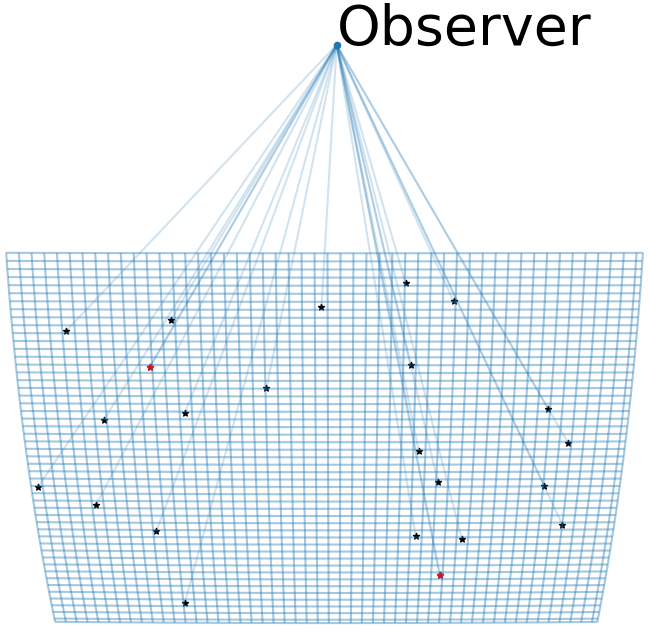
\includegraphics[scale=0.4]{images/benchmark.png}
    \caption{
    Visualization of an image presented to a star identification procedure.
    Stars are represented as vectors whose origin is the observer (i.e.\ Earth), and whose endpoint lies on a section
    of the celestial sphere.
    } \label{figure:benchmarkImageExample}
    }
\end{figure}

All stars from the catalog are selected such that no star exists more than $\frac{f}{2}$ away from the image center.
These stars and the image center are then rotated by $q_{rb}$ to construct the image stars.
The resulting image is presented in~\autoref{figure:benchmarkImageExample}.
What is presented to each identification method are the set of rotated catalog stars, the rotated image center, and
the field of view.

Noise is assumed to exist in two forms here: misrepresentations of the centroid (i.e.\ centroiding error and as
falsely identified sources of light in the image.
Centroiding error is applied to the rotated catalog star set by slightly rotating some star in this set, in some
random direction.
The severity is determined by a Gaussian distribution $N(0, \sigma^2)$.
False stars were added by generating a random vector within $\frac{f}{2}$ of the image center.

\subsection{What are the best hyperparameters for each algorithm?}\label{subsec:hyperparameterSelectionMethods}
This experiment helps determine the optimal hyperparameters (i.e.\ query $\sigma$, overlay $\sigma$) for each
identification method.
Referencing~\autoref{figure:genericIdentificationMethodFlowchart}, different values for this deviation in the
\textit{Search Catalog} step, or "query" step may lead to exclusion of the correct candidates in $R$.
Similarly, differing values for the overlay deviation in the \textit{Identify} step for methods using the
\Call{FPO} call may lead to the wrong map $a$ being selected.

The heuristic used to determine the optimal hyperparameters here was a grid search, iteratively exhausting every
permutation of some set of deviations and measuring the outcome of each trial.
The advantage of this heuristic is that every permutation is tested, but this comes at a cost of time and resources.
For this reason, a smaller number of trials were performed than that of the other experiments when determining
hyperparameters.

To determine the deviation for the query step, a permutation $P_n^{\sigma_n}$ is defined for some integer set $M$,
where:
\begin{equation}
    \label{eq:gridSearchQuery}
    \sigma_n \ \in \ \{ 10^{M_1}, 10^{M_2}, \ldots 10^{M_N} \}
\end{equation}
Each deviation above corresponds to some feature used to query the catalog.
For example, $n = 3$ for the Dot Angle method.
$\sigma_1$ corresponds to $\theta_{ic}$ in the query, $\sigma_2$ corresponds to $\theta_{jc}$, and $\sigma_3$
corresponds to $\phi$.

\begin{subequations}
    \label{eq:defineIdealQuery}
    For each output in~\autoref{eq:querySelectivityMeasures}, a deviation is considered ideal if all queries hit ($I_Q$)
    and have a sole element in the candidate set ($I_S$).
    \begin{align}
        I_Q(i) &=
        \begin{cases}
            1 & \text{if } \frac{Q_i}{N} = 1 \\
            0 & \text{otherwise}
        \end{cases} \\
        I_S(i) &=
        \begin{cases}
            1 & \text{if } \frac{S_i}{N} = 1\\
            0 & \text{otherwise}
        \end{cases}
    \end{align}
\end{subequations}

\begin{subequations}
    \label{eq:idealQuery}
    An ideal region length is the number of indicator variables ($I_Q, I_S$) for some
    consecutive deviation sequence.
    \begin{align}
        \text{Length of ideal } Q \text{ region } &= \sum_{i = 0}^N I_Q(i) \\
        \text{Length of ideal } S \text{ region } &= \sum_{i = 0}^N I_S(i)
    \end{align}
\end{subequations}

% Local Method: https://en.wikipedia.org/wiki/Sensitivity_analysis
\begin{subequations}
    \label{eq:sensitivityQuery}
    For the same outputs in~\autoref{eq:querySelectivityMeasures}, the sensitivity~\cite{SensitivityAnalysis}
    of some critical point $\sigma_c$ can be represented as:
    \begin{align}
        \left\lvert\frac{\partial Q}{\partial \sigma}\right\rvert_{\sigma_{c1}} &= \text{response of } Q \text{ to }
        \sigma \text{ at } \sigma_{c1} \\
        \left\lvert\frac{\partial S}{\partial \sigma}\right\rvert_{\sigma_{c2}} &=
        \text{response of } S \text{ to } \sigma \text{ at } \sigma_{c2}
    \end{align}
\end{subequations}

The more gradual the response is to the candidate set size or probability, the less penalizing an incorrect deviation
choice will be.
The longer that the responses above remain at zero, the less sensitive the hyperparameter selection is for that
specific feature.
The ideal feature set is one that has a long ideal period, and one with low responses to a deviation change.

To determine $\sigma$ for the identification step, the grid search devolves into a linear search.
$\sigma_o$ (overlay) is defined as~\autoref{eq:gridSearchQuery}, for some different set of $M$.

This deviation is used by the \Call{FPO}{} call, a function used by the Angle, Spherical Triangle,
Planar Triangle, and Composite Pyramid methods.
Given that this function operates the same for all identification methods above, this function was tested separately
as a binary classifier.
The sensitivity of this hyperparameter selection was characterized in terms of the resulting recall of the
classification:
\begin{equation}
    \label{eq:sensitivityIdentification}
    \left\lvert\frac{\partial \mathit{TPR}}{\partial \sigma}\right\rvert_{\sigma_o} = \text{response of } \mathit{TPR}
    \text{ at } \sigma_o \\
\end{equation}

Similarly, the longer the response above remains at zero the less sensitive the hyperparameter selection will be for
the \Call{FPO}{} call.

\subsection{Which set of features best distinguish a set of stars?}\label{subsec:querySelectivityMethods}
This experiment helps determine which identification method has the best querying process for catalog candidates $R$.
This is the first filter step, reducing the entire catalog to a subset of combinations.
If the correct stars do not exist here (filter produces false negatives), then the following steps will not be able to
correctly determine a map.
On the other hand if not enough of the catalog is filtered, there is a greater chance of error occurring at later steps.

Differences in catalog querying are specified in each paper (K-Vector, KD Trees, \ldots), but in this set of
experiments all catalog querying uses a B-Tree index.
The only unique portion of each query that remains are what features each method uses to search the catalog.
A general SQL statement to search each image star subset becomes:
\begin{align*}
    \texttt{SELECT } &r_1, r_2, \ldots, r_k \\
    \texttt{FROM } &C \\
    \texttt{WHERE } &(c_{f1} < q_{f1} + 3\sigma_1) \texttt{ AND } (c_{f1} > q_{f1} - 3\sigma_1) \texttt{ AND } \\
    &(c_{f2} < q_{f2} + 3\sigma_2) \texttt{ AND } (c_{f2} > q_{f2} - 3\sigma_2) \texttt{ AND } \\
    &\vdots \\
    &(c_{fn} < q_{fn} + 3\sigma_n) \texttt{ AND } (c_{fn} > q_{fn} - 3\sigma_n)
\end{align*}
\begin{align*}
    k =& \text{ number of stars used in the query.} \\
    c_f =& \text{ catalog feature amongst } r_1, r_2, \ldots, r_k.\\
    q_f =& \text{ image feature amongst an image star subset } b. \\
    n =& \text{ number of features used to query the catalog.} \\
    \sigma_n =& \text{ deviation of Gaussian noise.} \\
    C =& \text{ the catalog.}
\end{align*}

There are five features tested, given that Toloei's Composite Pyramid uses the same features as the Cole and
Crassidus's Planar Triangles method.
\begin{itemize}
    \item Angular separation $\theta^{ij}$ between two stars.
    \item Angular separations $\theta^{ic}, \theta^{jc}$ and dot angle $\phi$ between three stars.
    \item Planar area $a^{ijk}$ and moment $\imath^{ijk}$ between three stars.
    \item Spherical area $a^{ijk}$ and moment $\imath^{ijk}$ between three stars.
    \item Angular separations $\theta^{ij}, \theta^{ik}, \theta^{jk}$ between three stars.
\end{itemize}

\begin{subequations}
    \label{eq:querySelectivityMeasures}
    To quantify the selectivity and accuracy of each feature, we looked at:
    \begin{align}
        \text{Query hit probability } (Q) &= \frac{1}{N} \sum_{i = 0}^N y'(i) \\
        \text{Query selectivity } (S) &= \frac{1}{N} \sum_{i = 0}^{N} \lvert R(i) \rvert
    \end{align}

    Where $N$ is defined as the number of samples and $y'$ is defined as:
    \begin{equation}
        y' =
        \begin{cases}
            1 & \text{if correct star set } \in R \\
            0 & \text{otherwise}
        \end{cases}
    \end{equation}
\end{subequations}

The resulting candidate sets represents one element inside the \textit{set} of $R$ sets.
Repeating this $N$ times would give us the measures in~\autoref{eq:querySelectivityMeasures}.
$N = 2000$ here, and the entire experiment was repeated five times.

The running time of each query step $t$ (in seconds) will also be recorded.
This represents the time to retrieve each $R$ set, and will be used to determine the efficiency.
\begin{equation}\label{eq:queryEfficiency}
    \text{Query efficiency } = \frac{1}{|R| \times t}
\end{equation}

An ideal querying processes consists of a query hit probability = 1, a selectivity of 1 candidate set, and a high
efficiency.
The latter is desired as this reduces the amount of work required by the reduction process.

\subsection{What is the best process for reducing catalog candidates?}\label{subsec:candidateReductionMethods}
This experiment helps determine which identification method has the best querying + candidate reduction process.
If a reduction process is too restrictive, then a single match in $R$ will never be found.
If a reduction process is not restrictive enough, then the following steps will rarely determine a correct map.

For a majority of these methods, a reduction process is a matter of repeating the query steps until $\lvert R \rvert=1$
holds true.
For the triangle methods however, their reduction process is the \Call{Pivot}{} method.
The experiment reduces down to $\lvert R \rvert=1$ reduction vs. \Call{Pivot}{} reduction, coupled with each individual
method's query steps.

\begin{subequations}
    \label{eq:reductionAccuracyMeasures}
    To quantify the efficiency of each query + reduction process, we looked at:
    \begin{align}
        \text{Average reduction accuracy} &= \frac{1}{N} \sum_{i = 0}^N y''(i) \\
        \text{Average reduction running time} &= \frac{1}{N} \sum_{i = 0}^N t(i)
    \end{align}

    Where $t$ is defined as the running time to return one $r$ set and $y''$ is defined as:
    \begin{equation}
        y'' = \frac{| r \in \text{original, non-rotated image set}|}{|r|}
    \end{equation}
\end{subequations}

Referencing~\autoref{figure:genericIdentificationMethodFlowchart}, the experiment starts at the \textit{Get Camera
Image} step and executes the identification method to past the \textit{Confident in $r$?} decision block to produce a
single match from the catalog candidate set for some image star subset.
The resulting candidate set represent one element inside the set of $r$ sets.
Repeating this $N$ times would give us the measures in~\autoref{eq:reductionAccuracyMeasures}.
$N = 2000$ here, and the entire experiment was repeated five times.

An ideal reduction processes consists of a reduction hit probability = 1 and a short running time compared to the other
reduction processes.
We define the most efficient method as having the highest accuracy to running time ratio.

\subsection{Which method most accurately determines a map?}\label{subsec:identificationMethods}
This experiment helps determine which identification method produces the most accurate catalog to image maps.
An accurate map will reduce an attitude determination problem to Wahba's problem, which can be solved.

\begin{subequations}
    \label{eq:identificationAccuracyMeasures}
    To quantify the efficiency of each identification process (end-to-end), we looked at:
    \begin{align}
        \text{Average identification accuracy} &= \frac{1}{N} \sum_{i = 0}^N y'''(i) \\
        \text{Average identification running time} &= \frac{1}{N} \sum_{i = 0}^N t(i)
    \end{align}

    Where $t$ is defined as the running time to return a complete map and $y'''$ is defined as:
    \begin{equation}
        y''' = \frac{\text{number of correct mappings } b \rightarrow r}{\lvert b \lvert}
    \end{equation}
\end{subequations}

Referencing~\autoref{figure:genericIdentificationMethodFlowchart} again, this experiment runs the identification
method end to end.
Partial accuracy was recorded by counting the number of correct stars against the total amount of stars in a given
map.
$N = 2000$ here, and the entire experiment was repeated five times.

An ideal identification method consists of an average identification accuracy = 1 and a short running time compared
to the other identification methods.
We define the most efficient method as having the highest accuracy to running time ratio.
